\chapter{Preliminaries} \label{cha:Preliminaries}
This chapter details the requisite material for understanding the approach and implementation.

First, an overview of basic financial products and models are presented, as well as some risk measures. We then detail the concepts behind one of the most popular approaches to computational finance problems - Monte Carlo methods. Later, common methods for calculating sensitivities of financial products with respect to input parameters are described. Lastly, we touch on the application of GPUs to related problems and outline the CUDA architecture and its toolkit, followed by a brief review of other literature.

\section{Stochastic processes}
A stochastic process is a collection of random variables indexed by time, or alternatively, a probability distribution of a space of paths. In the following subsections we describe some specific cases of stochastic processes.

\subsection{Brownian motion}
A \textit{standard} Brownian motion over $[0,T]$ is a stochastic process $\{W(t), 0 \le t \le T\}$ with the following properties \cite{glasserman2004monte}:

\begin{enumerate}
    \item $W(0) = 0$;
    \item the mapping $t \mapsto W(t)$ is, with probability $1$, a continuous function on $[0,T]$;
    \item the increments $\{ W(t_1) - W(t_0), W(t_2) - W(t_1),\dots,W(t_k) - W(t_{k-1})\}$ are independent for any $k$ and any $0 \le t_0 < t_1 < \dots < t_k \le T$;
    \item $W(t) - W(s) \sim N(0, t-s)$ for any $0 \le s < t \le T$.
\end{enumerate}

We can see from properties $1$ and $4$ that 

\begin{equation}
    W(t) \sim N(0,t),
\end{equation}

for $0 < t \le T$.

We may also construct a Brownian motion $X(t)$ with a constant \textit{drift} $\mu$ and \textit{diffusion coefficient} $\sigma > 0$ as

\begin{equation*}
    X(t) = \mu t + \sigma W(t),
\end{equation*}

where the following is a standard Brownian motion: 

\begin{equation*}
    \frac{X(t) - \mu t}{\sigma}.
\end{equation*}

In Figure \ref{fig:standardbrownianmotion} three example paths of standard Brownian motion are shown.

\begin{figure}[h]
    \centering
    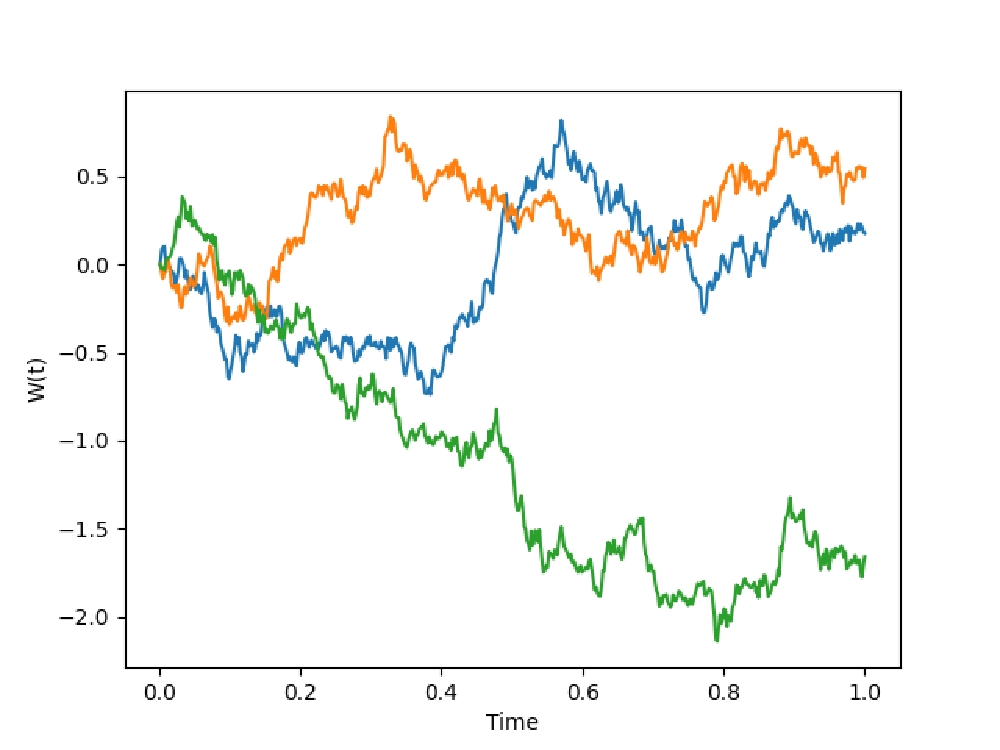
\includegraphics[width=0.8\textwidth]{figures/standard brownian motion.pdf}
    \caption{Three paths of a standard Brownian motion over $1$ year with $2^9$ equidistant timesteps.}
    \label{fig:standardbrownianmotion}
\end{figure}

\subsection{Martingales}
A stochastic process $X_t$ is known as a Martingale if 

\begin{equation*}
    E[X_t|\mathcal{F}_t] = X_s, \quad 0 \le s < t < \infty.
\end{equation*}

In other words, the conditional value of the next value in the sequence at any time $s$ is equal to the present value. If we use Martingales to model the price of an underlying asset, it means that all previous information about the price is available at the present time and we can disregard the past information. This fact, along with others, makes Martingales extremely useful in finance applications.

\section{Financial preliminaries}
\subsection{Derivatives}
Financial markets contain a wide range of products which are traded by market participants. One class of these products are known as \textit{derivatives}. A derivative is a contract whose value is derived from an asset, index, interest rate or other entity known as the "underlying". Derivatives are used for many purposes such as hedging risk or increasing exposure to underlying market changes and are ubiquitous in financial markets. Derivative contracts typically specify a set of conditions that define the obligations of the involved parties, important dates (such as expiration) and the notional value. Common types of derivatives are options, futures and swaps. 
Derivatives are of particular focus in computational finance as complex models which require high amounts of computation are needed to approximate their prices or sensitivities to input parameters.

\subsection{Options}
One of the most popular types of derivative is an option. An option is a contractual agreement which gives the owner, commonly referred to as the \textit{holder}, the right, but not the obligation, to buy or sell the underlying asset at a given price, the \textit{strike price} \(K\), on or before a specified expiration date \(T\). A European-style option only allows the holder to exercise the option at expiration time whereas an American-style option can be exercised at any time before expiration. For vanilla (simple) European-style options, a "call" option is one where the holder has the right to buy the underlying at expiration and a "put" allows them to sell the underlying at expiration.

According to the Black-Scholes model \cite{blackscholes}, the evolution of the stock price is described by the stochastic differential (SDE)

\begin{equation} \label{eqn:BlackScholesSDE}
    \frac{dS(t)}{S(t)} = r dt + \sigma dW(t),
\end{equation}

with \(W\) a standard Brownian motion. The parameters \(r\) and \(\sigma\) are the mean rate of return and volatility of the stock price respectively. $S(t)$ denotes the price of the underlying at time $t$. In the case where the mean rate of return is equal to the continuously compound interest rate \(r\) we are implicitly describing the \textit{risk-neutral} dynamics of the stock price. This idea is discussed extensively in literature and is core to the "fundamental theorem of asset pricing". The reader is referred to \cite{Dybvig2003} and Section 1.2.1 of \cite{glasserman2004monte} for further explanation.

The solution to the SDE in (\ref{eqn:BlackScholesSDE}) is

\begin{equation} \label{eqn:STsolution}
    S(T) = S(0)\exp{([r - \frac{1}{2}\sigma^2]T + \sigma W(T))}.
\end{equation}

With \(S(0)\) known, and the current price of the stock. If now is time \(t=0\) and at expiration time \(T\) the price of the underlying \(S(T)\) is greater than the strike price \(K\) then the holder exercises the option for a profit of \(S(T) - K\). Conversely, if the terminal price \(S(T)\) is less than \(K\) then the option expires worthless. Thus the payoff to the holder at expiration is given as

\begin{equation} \label{eqn:EuropeanCallPayoff}
    (S(T) - K)^+ = \max{\{0, S(T) - K\}}.
\end{equation}

There exist more complex options whose values are path-dependant and others with payoff functions that are not continuous. These properties pose extra challenges from an implementation perspective and continue to be a focal point in current literature.

\section{Monte Carlo methods} \label{sec:MonteCarloMethods}
\subsection{Principles of Monte Carlo} \label{sec:MonteCarloPriciples}
Monte Carlo methods, in the simplest form, rely on repeatedly taking random samples from a set of possible outcomes to determine the fraction of random draws which fall in a given set as an estimate of the set's volume in the probability space \cite{glasserman2004monte}. As the number of draws increases, the law of large numbers ensures the estimate converges to the true value and information about the magnitude of error in the estimate can be obtained through the central limit theorem.

Let us use the example from Section 1.1.2 of \cite{glasserman2004monte}, suppose we wish to calculate the expected present value of the payoff of a vanilla European call option on a stock. The payoff for this option is defined in (\ref{eqn:EuropeanCallPayoff}). Taking \(S(t)\) to be modelled as in (\ref{eqn:BlackScholesSDE}) thus giving the terminal price in (\ref{eqn:STsolution}), we can then draw samples from the distribution of the terminal stock price \(S(T)\) to calculate the expected value of the payoff \(E[e^{-rT}(S(T) - K)^+]\). As \(W(t)\) is a standard Brownian motion, the logarithm of the stock price is normally distributed. Thus we only need to draw random samples \(Z_i\) from the standard normal distribution to calculate \(S(T)\). Pseudocode is given below for estimating the expected present value of the payoff on the call option:

\begin{algorithm}[hbt!]
\caption{Algorithm to estimate expected present value of payoff}\label{alg:EstimateExpectedPayoff}
\begin{algorithmic}[1]
\For{$i \gets 1..n$}
    \State generate $Z_i$
    \State $S_i(T) = S(0)\exp{([r - \frac{1}{2}\sigma^2]T + \sigma \sqrt{T}Z_i)}$
    \State $C_i = e^{-rT}(S_i(T) - K)^+$
\EndFor
\State $\hat{C_n} = (C_1 + \dots + C_n) / n$
\end{algorithmic}
\end{algorithm}

This method can be generalised to calculate payoffs for more exotic path-dependent options and to other problems such as calculating the Greeks of a portfolio of derivatives - see \cite{giles2007monte} for further explanation.

\subsection{Pseudorandom number generation} \label{sec:prng}
Randomly sampling from probability distributions is the heart of Monte Carlo, so generating random samples quickly with sufficient "randomness" has been the topic of much research. The core of generating random samples in Monte Carlo is a \textit{pseudorandom number generator} (PRNG). PRNGs are deterministic algorithms that generate sequences of numbers whose properties mimic that of genuine random sequences. We do not attempt to cover PRNGs extensively; for a more detailed review of PRNG algorithms and their properties the reader is referred to \cite{l2010pseudorandom}, \cite{gu2016statistical} and Chapter 2 of \cite{glasserman2004monte}.
Most PRNGs used for Monte Carlo simulation are based on linear recurrences of the form

\begin{equation*}
    x_i = (a_1 x_{i-1} + \dots + a_k x_{i-k}) \mod{m},
\end{equation*}

where $k$ and $m$ are positive integers with $a_1 \dots a_k$ in $\{0, 1, \dots , m-1\}$ and $a_k \neq 0$. $m$ is typically a large prime number and the output is defined as $u_i = x_i / m$. The \textit{seed} of a generator is the initial set of values $x_{k-1}, \dots, x_0$.

There are several considerations which we take into mind when building PRNGs:
\begin{itemize}
    \item \textit{Good randomness properties}. A sequence of genuine random numbers $U_1, U_2, \dots$ satisfy the following properties:
    \begin{enumerate}
        \item Each $U_i$ is uniformly distributed between 0 and 1 (this is an arbitrary normalisation, any other range is acceptable).
        \item All $U_i$ are mutually independent.
    \end{enumerate}
    This is the hardest property to ensure for PRNGs but there has been enough examination of generators over time and those that are still in use today typically have passed statistical tests which show little deviation from truly random sequences.
    \item \textit{Large period}. The period of a PRNG is the minimum length of the output sequence before any number is repeated. Generators with large periods are key for use in simulation as we wish to draw millions of samples and without a sufficiently large period this would not be possible.
    \item \textit{Speed and efficiency of generation}. As we are generating millions of samples during a single simulation it is necessary for this process to be fast and require little effort computationally.
    \item \textit{Reproducibility}. It is important that using the same seed will result in the same output sequence. This allows us to run simulations multiple times with the same input to verify results.
\end{itemize}

\section{Quasi-Monte Carlo} \label{sec:quasimc}
Whereas Monte Carlo methods use pseudorandom sequences, Quasi-Monte Carlo (QMC) uses \textit{low-discrepancy sequences} (LDS). Rather than mimic randomness, LDS attempt to generate numbers that are evenly distributed. The advantage of using LDS is the rate at which they converge; Monte Carlo converges with rate $O(1/\sqrt{n})$, where $n$ is the number of paths, while QMC has convergence rate close to $O(1/n)$. 

The reliance on LDS however, leads QMC to have a dependence on the dimension of the problem and with many financial problems having high dimension due to large numbers of risk factors, time steps per path and the number of paths simulated, it is not guaranteed that QMC has greater performance over Monte Carlo. This has been addressed through a number of techniques such as \textit{variance reduction} \cite{allen2011variance}, \cite{WANGvariancereduction} and the concept of \textit{effective dimension} \cite{caflisch_1998}, \cite{WANGeffectivedim} may explain the success of QMC even for problems of high dimension.

To highlight the difference between QMC and Monte Carlo, let us consider the problem of numerical integration over the unit hypercube $[0, 1)^d$. We want to calculate

\begin{equation} \label{eqn:UnitHypercubeIntegral}
    E[f(U_1, \dots, U_d)] = \int_{[0,1)^d} f(x) dx,
\end{equation}

where $U_i$ are uniformly distributed random variables. This integral is approximated by

\begin{equation} \label{eqn:ApproxUnitHypercubeIntegral}
    \int_{[0,1)^d} f(x) dx \approx \frac{1}{n} \sum_{i = 1}^n{f(x_i)}.
\end{equation}

To calculate this value using Monte Carlo, we can construct a sequence $U_1, U_2, \dots$ and form vectors $(U_1, \dots, U_d), (U_{d+1}, \dots, U_{2d}), \dots$ which represents an i.i.d. sequence of points uniformly distributed on the unit hypercube. Here, we do not depend on the dimension $d$ to generate the sequence whereas the construction of points for QMC depends explicitly on the dimension, thus we cannot generate vectors of $d$ elements repeatedly. Rather we use LDS to choose points that effectively "fill" the hypercube as uniformly as possible. Common LDS include Sobol' sequences \cite{sobol1967distribution} and Halton sequences \cite{haltonsequences}.

\subsection{Van der Corput sequences} \label{sec:VanDerCorputSequences}
To talk in further detail about Sobol' sequences, we must introduce Van der Corput sequences. Following \cite{glasserman2004monte}, this sequence is a specific class of LDS in one dimension and is the core of many multidimensional constructions.

Every positive integer $k$ has what is known as it's base-$b$ representation such that

\begin{equation} \label{eqn:BaseBKRepresentation}
    k = \sum_{j=0}^{\infty}{a_j(k)b^j},
\end{equation}

where $b \ge 2$ and finitely many of the coefficients $a_j(k)$ are not equal to zero and in $\{0,1\dots,b-1\}$. The \textit{radical inverse function} $\psi_b$ is a mapping of each $k$ to $[0,1)$ and is given as

\begin{equation} \label{eqn:RadicalInverseFunction}
    \psi_b(k) = \sum_{j=0}^{\infty}{\frac{a_j(k)}{b^{j+1}}}.
\end{equation}

The Van der Corput sequence in base-$b$ is $0 = \psi_b(0), \psi_b(1), \psi_b(2),\dots$ and we give the sequence in base $2$ below.

\begin{table}[!h]
\centering
$\begin{array}{ c c c c } 
 \hline
 k & k\;\text{Binary} & \psi_2(k)\;\text{Binary} & \psi_2(k) \\
 \hline
 0 & 0   & 0     & 0 \\
 1 & 1   & 0.1   & 1/2 \\
 2 & 10  & 0.01  & 1/4 \\
 3 & 11  & 0.11  & 3/4 \\
 4 & 100 & 0.001 & 1/8 \\
 5 & 101 & 0.101 & 5/8 \\
\end{array}$
\caption{Radical inverse function $\psi_b$ in base $2$.}
\label{tbl:RadicalInverseBase2}
\end{table}

Table \ref{tbl:RadicalInverseBase2} shows how the sequence fills the unit interval; the $k$th row shows the first $k$ nonzero elements of the sequence and each row refines the previous one. The Van der Corput sequence also fills the points in a maximally balanced way. For example following the final row of Table \ref{tbl:RadicalInverseBase2} we would fill $1/16$, then $9/16$, then $5/16$ and so on. The values alternate either side of $1/2$, then either side of $1/4$ and this continues. An important property to note is that the larger the base $b$, the greater the number of points required to reach uniformity.

\subsection{Sobol' sequences} \label{sec:SobolSequences}
First introduced by Sobol' in 1967 \cite{sobol1967distribution}, was the construction of a $(t,d)$-sequence. Sobol's construction can be contrasted with other LDS such as Faure's \cite{Faure1982} as Faure's points are $(0,d)$-sequences in a base at least as large as $d$ whereas Sobol's points are $(t,d)$-sequences in base $2$ for all $d$, with values of $t$ that depend on $d$ \cite{glasserman2004monte}. This gives Sobol' points the advantage of a much smaller base but with slightly less uniformity. The ability to work in base $2$ has obvious advantages when applied to the computational setting with bit-level operations.

The Sobol' points start from the Van der Corput sequence in base $2$ only and the coordinates of a $d$-dimensional sequence come from permutations of sections of the Van der Corput sequence. These permutations result from the product of binary expansions of consecutive integers with a set of generator matrices, one for each dimension. A generator matrix $\boldsymbol{G}$ has columns of binary expansions of a set \textit{direction numbers} $g_1,\dots,g_r$ with elements equal to $0$ or $1$. The value $r$ represents the number of terms in the binary expansion of $k$ and can be arbitrarily large. Let $(a_0(k),\dots,a_{r-1}(k))^\top$ represent the vector of coefficients of the binary representation of $k$ such that

\begin{equation} \label{eqn:GeneratorMatrixExpression}
    \begin{pmatrix}
    y_1(k) \\
    y_2(k) \\
    \vdots \\
    y_r(k)
    \end{pmatrix}
    = \boldsymbol{G} 
    \begin{pmatrix}
    a_0(k) \\
    a_1(k) \\
    \vdots \\
    a_{r-1}(k)
    \end{pmatrix}
    \mod{2},
\end{equation}

and $y_1(k),\dots,y_r(k)$ are the coefficients of the binary expansion of the $k$th point in the sequence. This gives the $k$th point as:

\begin{equation*}
    x_k = \frac{y_1(k)}{2} + \frac{y_2(k)}{4} + \dots + \frac{y_r(k)}{2^r}.
\end{equation*}

The generator matrix $\boldsymbol{G}$ is upper triangular and the special case where it is the identity matrix results in the Van der Corput sequence in base $2$. We can perform (\ref{eqn:GeneratorMatrixExpression}) in a computer implementation through a bitwise XOR operation, giving us the computer representation of $x_k$ as

\begin{equation*}
    a_0(k)g_1 \oplus a_1(k)g_2 \oplus \dots \oplus a_{r-1}(k)g_r,
\end{equation*}

where $\oplus$ is the bitwise XOR operator.

The core of the Sobol' method are the generator matrices $\boldsymbol{G}$ and their direction numbers $g_j$. As previously mentioned, we require $d$ sets of direction numbers to produce a $d$-dimensional sequence. The method begins by selecting a \textit{primitive polynomial} over binary arithmetic. The polynomial

\begin{equation} \label{eqn:SobolPrimitivePolynomial}
    x^q + c_1x^{q-1} + \dots + c_{q-1}x + 1,
\end{equation}

has coefficients $c_i$ in $\{0,1\}$ and satisfies two properties \cite{glasserman2004monte}:

\begin{itemize}
    \item it cannot be factored;
    \item the smallest power $p$ for which the polynomial divides $x^p + 1$ is $p = 2^q - 1$.
\end{itemize}

The primitive polynomial in (\ref{eqn:SobolPrimitivePolynomial}) defines a recurrence relation

\begin{equation} \label{eqn:SobolRecurrenceRelation}
    m_j = 2c_1m_{j-1} \oplus 2^2c_2m_{j-2} \oplus \dots \oplus 2^{q-1}c_{q-1}m_{j-q+1} \oplus 2^qm_{j-q} \oplus m_{j-q},
\end{equation}

where the $m_j$ are integers. We define the directions numbers as

\begin{equation*}
    g_j = \frac{m_j}{2^j}.
\end{equation*}

Of course, to fully define the direction numbers we need initial values for $m_1,\dots,m_q$. It is enough to set each initialising $m_j$ to be an odd integer less than $2^j$, which ensures that all following $m_j$ as defined by (\ref{eqn:SobolRecurrenceRelation}) also share this property. From this, each $g_j$ will be strictly between $0$ and $1$.

So, to construct a sequence we take the primitive polynomial and use the recurrence relation (\ref{eqn:SobolRecurrenceRelation}) with some initial $m_j$. We then calculate the corresponding direction numbers $g_j$ by dividing by $2^j$ (or performing a binary shift of the binary point $j$ places to the left). Then with these direction numbers we construct the generator matrix $G$. With this generator matrix we take a vector $\boldsymbol{a}(k)$ of binary coefficients of $k$ and perform the operation in (\ref{eqn:GeneratorMatrixExpression}) to give us the coefficients of a binary fraction, from which we obtain $x_k$.

There has been much research on choosing initial direction numbers, and also more efficient construction implementation (namely Gray code construction \cite{GrayCodeConstruction}), which we will not go into further detail about.

\subsection{Scrambled Sobol'} \label{sec:ScrambledSobol}
As we are choosing points deterministically we are unable to measure error through a confidence interval. In sacrificing some of the accuracy obtained through careful selection of points, randomised QMC points allow us to calculate this error. One method for producing randomised QMC points is known as \textit{scrambling}.

Introduced by Owen and further developed in \cite{OwenScrambling}, scrambling is a technique that permutes each digit of a $b$-ary expansion, where the permutation applied to the $j$th digit is dependent on the preceding $j-1$ digits. Scrambling can be described by taking each coordinate, partitioning the unit interval into $b$ subintervals of length $1/b$ and then randomly permuting those subintervals. Then, further partition each subinterval into $b$ subintervals of length $1/b^2$ and permute those, and so on. At the $j$th step, we have $b^{j-1}$ partitions, each of which consist of $b$ intervals, and each is permuted randomly and independently.

\section{Graphics Processing Units and CUDA}
The Graphics Processing Unit (GPU) has seen widespread adoption in computational finance due to its highly parallel architecture designed for increased computational throughput. When NVIDIA released CUDA \cite{cudazone} in 2007 it enabled more "general-purpose" usage of the previously graphics-focused applications of GPUs.

\subsection{CUDA architecture} \label{sec:cudaarch}
The CUDA architecture allows each and every arithmetic logic unit (ALU) on the chip to be marshaled by a program \cite{sanders2010cuda}. It is implemented by organising the the GPU into a collection of \textit{streaming multiprocessors}, which operate following the Single-Instruction-Multiple-Thread (SIMT) paradigm. Because of the intended usage for general-purpose computation CUDA allows for arbitrary read and write access to memory and the software-managed cache known as \textit{shared memory}.

From a software perspective, the CUDA architecture allows for \textit{kernels} to be ran in parallel across a \textit{grid}. This grid is composed of multiple \textit{blocks}, each of which contains a collection of threads which all run the program defined by some launched kernel. Both blocks and grids can have up to three dimensions each and CUDA provides useful syntax for indexing into them. In hardware, the threads inside of a block are grouped into sets of 32 threads known as a \textit{warp}, where all threads inside the same warp execute the same instruction.

\begin{figure}[h]
    \centering
    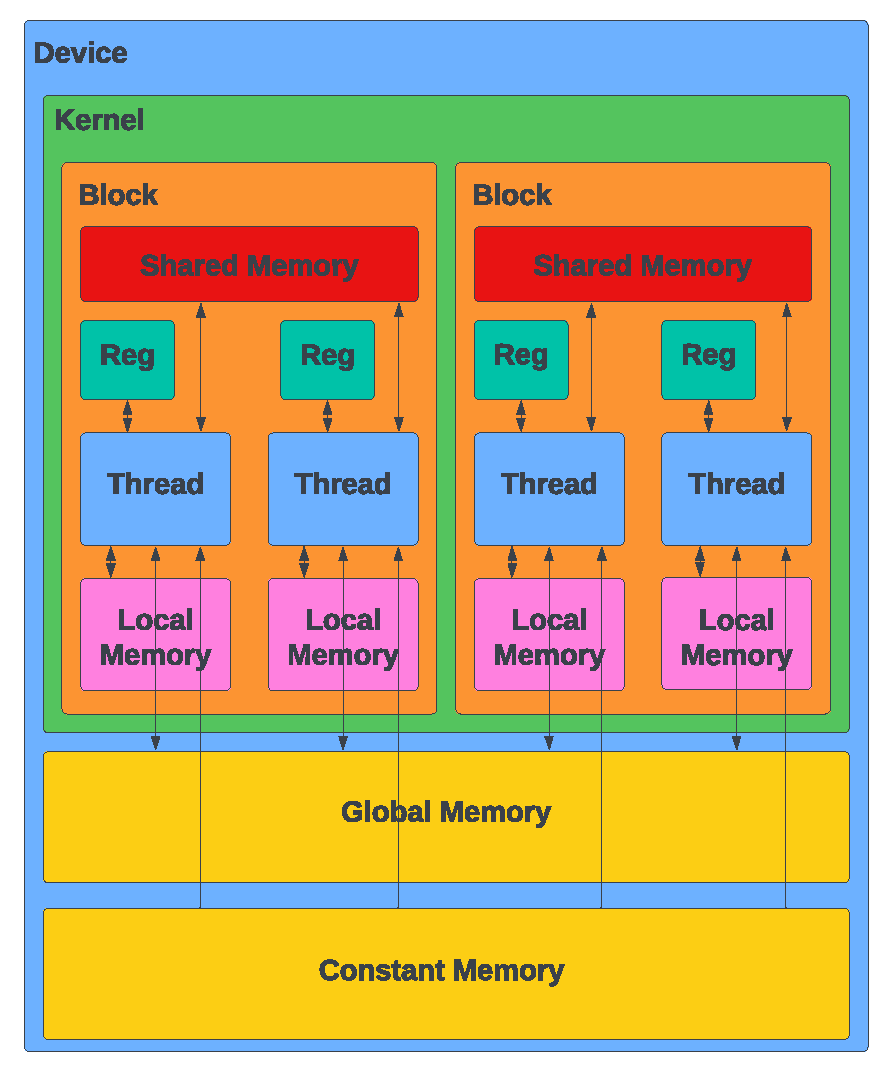
\includegraphics[width=0.6\textwidth]{figures/cuda arch.pdf}
    \caption{Basic CUDA memory architecture. Inspired by https://cvw.cac.cornell.edu/gpu/memory\_arch}
    \label{fig:cudaarch}
\end{figure}

Each thread has its own local memory and registers, and threads in the same block have access to the on-chip shared memory of that block. This is often how threads within a block communicate with each other while maintaining high performance. The basic architecture is shown in Figure \ref{fig:cudaarch}.

NVIDIA have also developed a toolkit for CUDA \cite{cudatoolkitdocumentation} which contains the compiler, highly parallel implementations of mathematical libraries (such as cuBLAS, cuRAND and cuFFT) and a host of other useful tools like a debugger and memory checker.

\subsection{Practical implementation considerations}
There are many considerations one must take into account when implementing algorithms on a GPU. Most notably, the limited size of on-chip caches in comparison to the relatively large size of global memory. For financial problems with high dimensions (such as Monte Carlo simulations of many paths or many assets) shared memory will quickly become a limiting factor to the speed of an implementation. This is because reading from global memory is roughly 100x slower than loading directly from shared memory. This limitation has been addressed in literature and a few common design patterns have arisen such as pre-computation of values shared between threads, merging of kernels to avoid redundant data transfers and using coalesced reads and writes. See \cite{dixon2012monte} for an example of how problem reformation can lead to large speed ups and see \cite{BrodtkorbGPU} for further discussion of GPU programming strategies.